\section{Introduction}
%%%%%%%%%%%%%%%%%%%%%%%%%%%%%%%%%%%%%%%%%%%%%%%%%%%%%%%%%%%%%%%%%%%%%%%%%%%%%%%%
%%%%%%%%%%%%%%%%%%%%%%%%%%%%%%%%%%%%%%%%%%%%%%%%%%%%%%%%%%%%%%%%%%%%%%%%%%%%%%%%
\subsection{Motivation: The problem we are solving}
\hl{TODO problem statement}
%%%%%%%%%%%%%%%%%%%%%%%%%%%%%%%%%%%%%%%%%%%%%%%%%%%%%%%%%%%%%%%%%%%%%%%%%%%%%%%%
\subsubsection{Benchmarks}
\subsubsection{USB}
electrical characteristics: maximum $500 \myunit{mA}$ @ fixed $5 \myunit{V}$ DC ($5 \myunit{W}$ power handling)
\subsubsection{Benchtop power supply}
electrical characteristics: maximum $3 \myunit{A}$ @ variable $0 - 30 \myunit{V}$ DC ($90 \myunit{W}$ power handling)
~\\
physical characteristics: product weight $7 \myunit{kg}$; $\sim 0.01 \myunit{m}^3$
Maybe cost? 430 for the one we have in the lab:  https://core-electronics.com.au/laboratory-dc-power-supply-2x-outputs-at-0-30v-3a.html
%%%%%%%%%%%%%%%%%%%%%%%%%%%%%%%%%%%%%%%%%%%%%%%%%%%%%%%%%%%%%%%%%%%%%%%%%%%%%%%%
%%%%%%%%%%%%%%%%%%%%%%%%%%%%%%%%%%%%%%%%%%%%%%%%%%%%%%%%%%%%%%%%%%%%%%%%%%%%%%%%
\subsection{Background Theory - The 2 subsystems of a charge management system}

ADD INTRODUCTION PARAGRAPH HERE

\subsubsection{An introduction to ultra-capacitors}
Electrochemical double layer capacitor(EDLCs) is also known as ultra-capacitors. It is a type of capacitor with higher power density than conventional capacitor and higher energy density than batteries. Due to such high capacitance, ultra-capacitors are used as energy storage in applications. \cite{maxwell}, \cite{murata}. 

An ultra-capacitor is typically composed of two electrodes coated with activated carbon powder, electrolytes and a separator in between them. Due to activated carbon, they have much bigger surface area allowing more energy to be stored. 

In comparison to batteries, ultra-capacitors have much smaller Equivalent Series Resistance (ESR). This allows high current charging and discharging as well as high power density. So ultra-capacitors are suitable for low power and high power applications, whereas batteries only suitable for low power applications. Due to such high power density, the size of ultra-capacitor is much smaller. However, as a result of low ESR, the stored energy will be released quickly when short-circuited and might cause electric arcing \cite{murata}. Hence care must be taken to limit the current. 

Like a battery, ultra-capacitors also have voltage limits. It can only withstand low voltage, usually 2.7V. Larger voltage can be applied when capacitors are connected in series however balancing is required as over-voltage protection. 

While battery remains at approximately constant voltage until they are depleted, the voltage across ultra-capacitor decreases linearly when a constant current is drawn, refer to Figure \ref{fig:comparison}. Hence additional circuitry to maintain constant voltage is required for ultra-capacitor to act as a battery. 

\begin{figure}
    \centering
    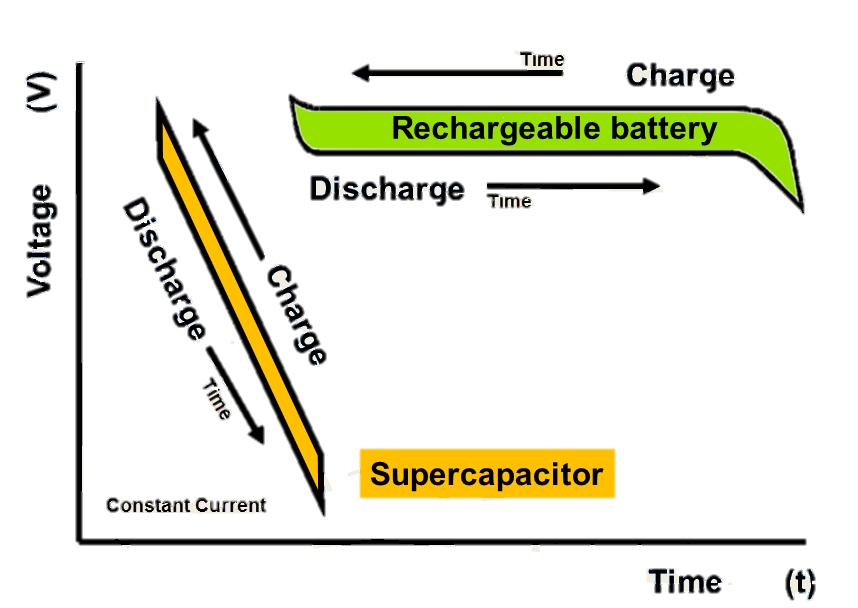
\includegraphics[width=0.7\textwidth]{figures/ChargeDischarge.png}
    \caption{Ultra-capacitor vs Battery \cite{ultracap_fig}}
    \label{fig:comparison}
\end{figure}

%%%%%%%%%%%%%%%%%%%%%%%%%%%%%%%%%%%%%%%%%%%%%%%%%%%%%%%%%%%%%%%%%%%%%%%%%%%%%%%%
\subsubsection{An introduction to DC-DC converters}
Switched-mode DC-DC converters provide a method for converting a DC input voltage to a DC output voltage of greater or lesser magnitude by the use of 3 fundamental components: a switch; a diode; and an energy storage component. This energy storage component may achieve its function through storage in magnetic field (i.e. inductors) or through storage in electric field (i.e. capacitors). MOSFETs are typically used to achieve the switching behaviour.
\newpar
A sub-class of DC-DC converters are those that can produce an output voltage that is either greater (termed `boost' behaviour) or lesser (termed `buck' behaviour) in magnitude than the input voltage. Such converters are termed `buck-boost' converters. The nature of the switching signal applied to the buck-boost converter determines the mode of operation and is typically of pulse-width modulation (PWM) form. For a typical converter, a PWM signal that is on for a shorter proportion of time than it is off produces buck behaviour and a PWM signal that is on for a longer proportion of time than it is off produces boost behaviour.
\newpar
Buck-boost converters are favoured for their very high efficiency and simplicity of implementation. They exist nearly everywhere where an output DC voltage of greater or lesser magnitude than a DC input voltage is required to be generated.
%%%%%%%%%%%%%%%%%%%%%%%%%%%%%%%%%%%%%%%%%%%%%%%%%%%%%%%%%%%%%%%%%%%%%%%%%%%%%%%%
%%%%%%%%%%%%%%%%%%%%%%%%%%%%%%%%%%%%%%%%%%%%%%%%%%%%%%%%%%%%%%%%%%%%%%%%%%%%%%%%
\subsection{What a solution would look like}\label{sec:solution}
\begin{itemize}
    \item where power comes from
    \item where control occurs
    \item what measured
    \item what controlled
\end{itemize}
%%%%%%%%%%%%%%%%%%%%%%%%%%%%%%%%%%%%%%%%%%%%%%%%%%%%%%%%%%%%%%%%%%%%%%%%%%%%%%%%
%%%%%%%%%%%%%%%%%%%%%%%%%%%%%%%%%%%%%%%%%%%%%%%%%%%%%%%%%%%%%%%%%%%%%%%%%%%%%%%%
\subsection{The delivered product}
\subsubsection{Pictures}
\subsubsection{System diagram}
\subsubsection{Control flow}
\tikzstyle{block} = [rectangle, draw, fill = \myblue, text width=5em, text badly centered, rounded corners, minimum height=4em]
\tikzstyle{line} = [draw, -latex']
\begin{figure}[H]
\centering
\fbox{
\begin{tikzpicture}[node distance = 3cm]
\node [block, fill = \myorange] (cuk) {DC-DC converter};
\node [block, right = of cuk, fill = \myblue] (load) {load};
\node [block, left = of cuk, fill = \myblue] (caps) {ultra-capacitors};
\node [block, below = of cuk, fill = \mygreen] (uC) {micro-controller};
\node [block, below = of uC, fill = \myblue] (USB) {USB};
%
\path [line, ultra thick] (caps)
	--
	node [anchor = south, align = center]
	{input voltage}
    (cuk);
\path [line, ultra thick] (caps)
    to[out = -90, in = 180]
	node [anchor = east, align = center]
	{input voltage}
    (uC);
\path [line, ultra thick] (uC)
	--
	node [anchor = west, align = center]
	{PWM duty ratio}
    (cuk);
\path [line, ultra thick] (cuk)
	--
	node [anchor = south, align = center]
	{output voltage}
    (load);
\path [line, ultra thick] (load)
    to[out = -90, in = 0]  
	node [anchor = west, align = center]
	{output voltage}
    (uC);
\path [line, ultra thick] (USB)
    to[out = 110, in = -110]
	node [anchor = east, align = center]
	{reference voltage}
    (uC);
\path [line, ultra thick] (uC)
    to[out = -70, in = 70] 
	node [anchor = west, align = center]
	{input voltage, \\ output voltage, \\ PWM duty ratio}
    (USB);
\end{tikzpicture}
}
\caption{Control flow diagram of product}
\label{fig:controlflow}
\end{figure}
\tikzstyle{block} = [rectangle, draw, fill=\myblue, 
text width=5em, text badly centered, rounded corners, minimum height=4em]
\tikzstyle{smallblock} = [rectangle, draw, fill=\myblue, 
text width=3em, text badly centered, rounded corners, minimum height=3em]
\tikzstyle{line} = [draw, -latex']
\begin{figure}[H]
\centering
\fbox{
\begin{tikzpicture}[node distance = 3.5cm]
    \node [block, fill = \myorange] (cuk) {DC-DC converter};
    \node [block, right = of cuk, fill = \myblue] (load) {load};
    \node [block, left = of cuk, fill = \myblue] (caps) {ultra-capacitors};
    %
    \node [smallblock, below = 2cm of cuk, fill = \mygreen] (PWM) {\small PWM};
    \node [smallblock, below = 2cm of PWM, fill = \mygreen] (control) {\small control loop};
    \node [smallblock, left = 2cm of control, fill = \mygreen] (ADC1) {\small ADC};
    \node [smallblock, right = 2cm of control, fill = \mygreen] (ADC2) {\small ADC};
    \node [smallblock, below = 2cm of control, fill = \mygreen] (UART) {\small UART};
    %
    \node [block, below = 3cm of UART, fill = \myblue] (USB) {USB};
    %
    \node [above left = -0.5cm and 1cm of PWM] (uC) {microcontroller};
    %
    \path [line, ultra thick] (caps)
    --
    node [anchor = south, align = center]
    {input voltage}
    (cuk);
    %
    \path [line, ultra thick] (caps)
    to[out = -90, in = 180]
    node [anchor = east, align = center]
    {input voltage}
    (ADC1);
    %
    \path [line, ultra thick] (PWM)
    --
    node [anchor = west, align = center]
    {PWM \\ at calculated duty ratio}
    (cuk);
    %
    \path [line, ultra thick] (cuk)
    --
    node [anchor = south, align = center]
    {output voltage}
    (load);
    %
    \path [line, ultra thick] (load)
    to[out = -90, in = 0]
    node [anchor = west, align = center]
    {output voltage}
    (ADC2);
    %
    \path [line, ultra thick] (USB)
    to[out = 110, in = -110]
    node [anchor = east, align = center]
    {reference voltage}
    (UART);
    %
    \path [line, ultra thick] (UART)
    to[out = -70, in = 70]
    node [anchor = west, align = center]
    {input voltage, output voltage, \\ estimated state variables, PWM duty ratio}
    (USB);
    %
    \path [line, ultra thick] (ADC1)
    --
    node [anchor = south, align = center]
    {input \\ voltage}
    (control);
    %
    \path [line, ultra thick] (ADC2)
    --
    node [anchor = south, align = center]
    {output \\ voltage}
    (control);
    %
    \path [line, ultra thick] (control)
    --
    node [anchor = center, align = center, above right = 0cm and 0cm]
    {duty ratio}
    (PWM);
    %
    \path [line, ultra thick] (UART)
    to[out = 110, in = -110]
    node [anchor = east, align = center]
    {reference}
    (control);
    %
    \path [line, ultra thick] (control)
    to[out = -70, in = 70]
    node [anchor = west, align = center]
    {voltages, state variables, \\ PWM duty ratio}
    (UART);
    % background
    \begin{pgfonlayer}{background}
    	\draw[thick, rounded corners, fill = yellow!30, draw = black, dashed] ($(ADC1) + (-1.6, 4.2)$) rectangle ($(ADC2) + (1.6, -4.4)$);
    \end{pgfonlayer}
\end{tikzpicture}
}
\caption{Alternative control flow diagram of product}
\label{fig:controlflow2}
\end{figure}
\subsubsection{Specifications}
physical characteristics: $\sim 0.3 \myunit{kg}$; $\sim 0.0006 \myunit{m}^3$
\begin{itemize}
    \item transient performance
\end{itemize}
%%%%%%%%%%%%%%%%%%%%%%%%%%%%%%%%%%%%%%%%%%%%%%%%%%%%%%%%%%%%%%%%%%%%%%%%%%%%%%%%
%%%%%%%%%%%%%%%%%%%%%%%%%%%%%%%%%%%%%%%%%%%%%%%%%%%%%%%%%%%%%%%%%%%%%%%%%%%%%%%%
\begin{comment}
\subsection{Project Aim}
\begin{itemize}
    \item Ultra-capacitor charge and discharge characteristics must be well described
    \item DC-DC converter must reject ramp disturbances entering at the input voltage
    \item control loop must produce zero steady-state error from reference
    \item system must be safe under normal and extreme operating operating conditions
    \item control loop must be robust
    \item entire system must be charged/powered, and communicate through USB
\end{itemize}
\end{comment}
%%%%%%%%%%%%%%%%%%%%%%%%%%%%%%%%%%%%%%%%%%%%%%%%%%%%%%%%%%%%%%%%%%%%%%%%%%%%%%%%
%%%%%%%%%%%%%%%%%%%%%%%%%%%%%%%%%%%%%%%%%%%%%%%%%%%%%%%%%%%%%%%%%%%%%%%%%%%%%%%%
%%%%%%%%%%%%%%%%%%%%%%%%%%%%%%%%%%%%%%%%%%%%%%%%%%%%%%%%%%%%%%%%%%%%%%%%%%%%%%%%